\section{GPU}
\label{sec:cuda}

The development of a GPU implementation of \polu was divided into two phases.
The initial implementation consisted only on getting a working implementation, with basic, somewhat naive kernels implemented to move \computeflux and \update computations to the GPU.
After a comparison with the other implementation done at that point, it was decided to invest more time in the CUDA version.
Not only was its execution time much better than other implementations, since it was still a naive implementation it was most likely to still have room for improvements.

\subsection{Load Balance}
\label{subsec:cuda:load}

\todo[inline,color=green!40]{Explain how the workload is assigned to each thread}

\subsection{Optimizations}
\label{subsec:cuda:load}

One of the first optimizations done comes from a simplification already explained in \todo[inline]{Onde é que explicas que a reduction pode ser feita fora do loop?}. The initial implementation, like the CPU versions, relied on a reduction to compute the maximum velocity after each iteration. The reduction used was based on the most optimized implementation provided in the NVidia samples, and is, according to the author, one of the most optimized CUDA reductions.

But the simplification of moving the maximum velocity computation to outside of the loop didn't rely only on the reduction, as that was only the final step of the computation. There was also added workload to the \computeflux kernel, which had to compute the velocity in each CUDA thread. More than the amount of operations, this had a considerable impact on the amount of registers used by the kernel, and it was noted that after its removal, there was also some improvements in \computeflux, and consequentely, in the main loop. This can be seen in \cref{fig:time_computeflux}.

\subsubsection{Second Phase}
\label{subsubsec:cuda:load:second}

On the second phase of the development of a CUDA implementation, more attention was given to the individual performance of the kernels. A lot of experiments were done with different kernel implementations, in order to test different approaches to eliminate memory accesses, and reduce or eliminate divergent branches.

While this provided small improvements to kernel execution time, consequentely decreasing the main loop time considerably, the better speedup was achieved after a division operation was removed from the \update, which computed a ratio between the length of an edge and the area of a cell. This was achieved by precomputing a matrix with the value of the ratio prior to the main loop. This required a considerable  amount of additional memory to be used on the GPU, but since the problem is not bound by total size (biggest test case used consisted of less than 100MB) and division operations are very costly to a GPU, this showed large improvements for the \update kernel, as shown in \cref{fig:time_update}

\begin{figure}[!htp]
	\begin{subfigure}[b]{\columnwidth}
		\centering
		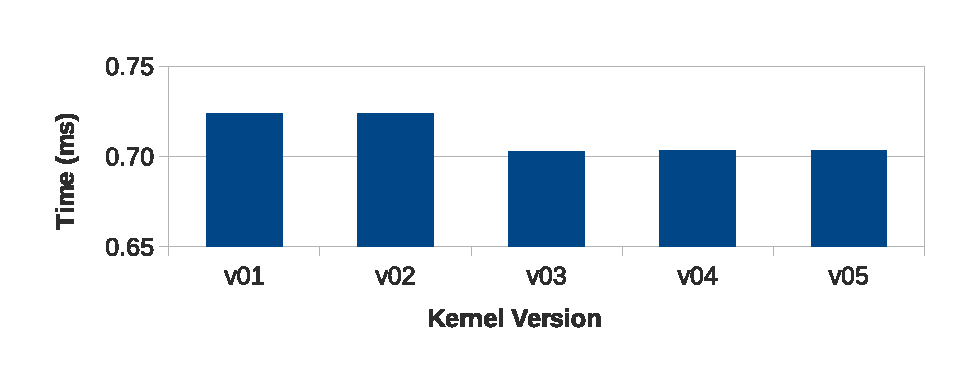
\includegraphics[width=\columnwidth]{graph_compute_flux}
		\caption{\computeflux}
		\label{fig:time_computeflux}
	\end{subfigure}
	\begin{subfigure}[b]{\columnwidth}
		\centering
		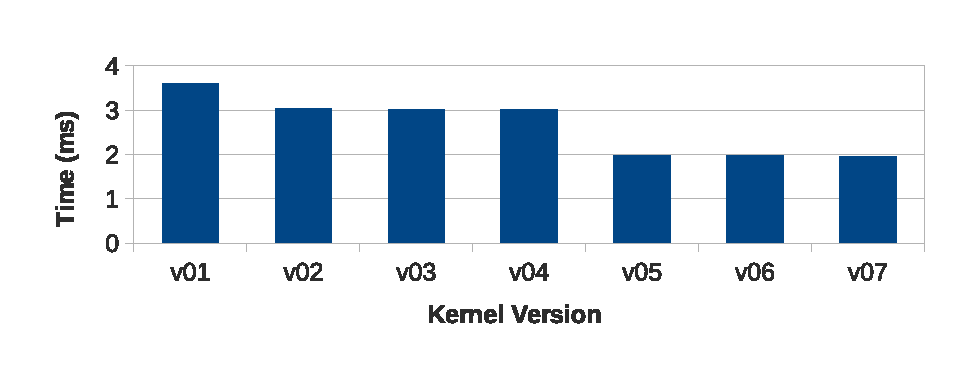
\includegraphics[width=\columnwidth]{graph_update}
		\caption{\update}
		\label{fig:time_update}
	\end{subfigure}

	\caption{Indivudual kernel speedups. Times are the average for a single kernel call}
	\label{fig:time_kernels}
\end{figure}

Times shown in \cref{fig:time_kernels} were measured using the CUDA Events API, which allows measurements of GPU events, excluding the callback overhead of issuing a kernel call. That, along with the fact that both kernels have considerably short and simple code, explains the low times, even for the initial versions. Even so, the removal of the division operation, along with other smaller tweaks, allowed the execution time of the \update kernel to be almost halved.

Due to the low precision of the measurements when compared to the small execution time of the kernels\footnote{CUDA Events API only claims a precision of 0.5 ms}, no immediate changes can be seen between some of the versions. However, since later kernels are the result of aggregating most optimizations from previous versions, intermediate results are still shown.

\subsection{Mesh ordering impact}
\label{subsec:cuda:ordering}

\todorev{Last revised on Sun, July 1 at 00:15 by pfac}

Since GPUs rely heavily on memory organization, it comes as no surprise that the issues stated at \cref{sec:omp:limitations}, and shown in \cref{fig:locality} become even more relevant.

Memory accesses in a GPU are more efficient when the data being accessed at the same time is contiguous in memory, allowing for a single, coalesced memory request to be issued. The lack of locality provided by \texttt{gmsh} output, as well as the irregular memory access pattern from each kernel complicates this task.

A simple approach was taken to attempt minimizing this problem, which consisted on preprocessing the mesh, moving all cells in the border to the beginning of the structure.
The idea was not to increase locality, since the border is only a small subset of the entire mesh, but to attempt more regular accesses in \computeflux, as well as avoiding the divergent branch for border cells.
With all border cells being sequential, then only a single warp should diverge on the branch which tests borders.

This solution showed no visible improvements, probably due to the already extremely low kernel execution times, which become bottlenecked by the kernel callback overhead. 

\subsection{Results}
\label{subsec:cuda:results}

Results for the CUDA implementations are here presented in the form of speedups, relatively to the original raw version of \polu (see \cref{sec:method} for details on the testing methodology). Results were measured by comparing both the first, more naive CUDA implementation, and the last implementation, with better kernels and the divison removed from \update kernel. . Some intermediate implementantions were also created, since optimizations were agregated by each new kernel version created, but only the final results of the optimizations are shown here, in \cref{fig:cuda:results}

\begin{figure}[!htp]
	\centering
	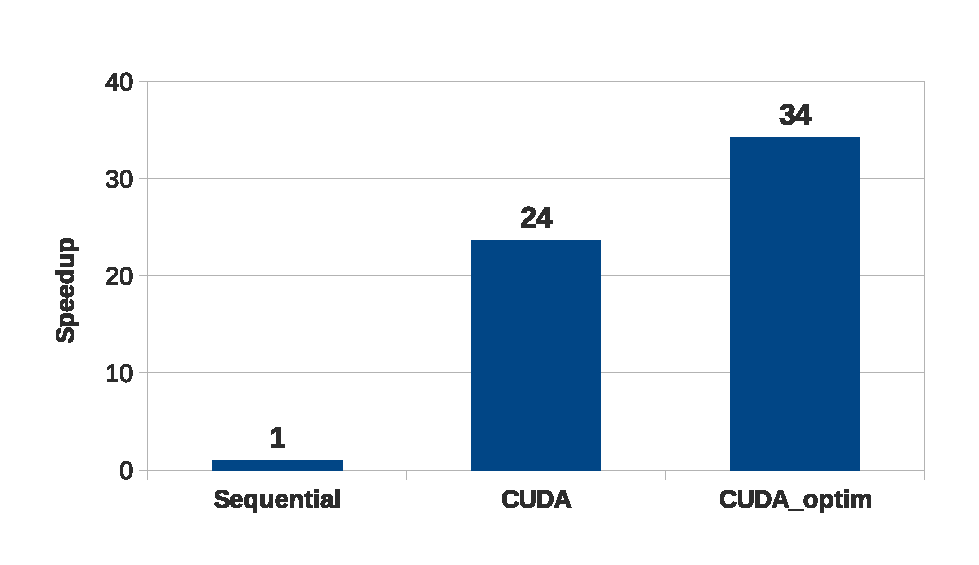
\includegraphics[width=\columnwidth]{graph_comparison_cuda}
	\caption{CUDA implementation speedups}
	\label{fig:cuda:results}
\end{figure}

The initial CUDA version already showed significant performance gains, almost matching the best speedup achieved with the OpenMP implementation in \cref{sec:omp}. Optimizations were able to boost this speedup even further, achievent a total speedup of 34, the best one achieved in this work.
However, the gain against the OpenMP version is not as large as previously expected, since this problems seems extremelly well suited to a massively parallel approach, like the one employed by CUDA. This is a result of the limited test case size, which was generated using a conversion utility provided with \polu, that converts \texttt{gmsh} output to a XML file readable by \polu. This utility was not subject to optimizations or parallelization, but uses an algorithm in the order of $\Theta(N^3)$, making the generation of larger test cases impossible due to time limitations. The test cases available, which only go up to 62MB, still do not reach the maximum capacity of the GPU, which may even benefit from the addition of even more threads.

Given the chance to test this theory, this could show much greater scalability for the CUDA implementation.


